\documentclass[11pt]{scrartcl}
\usepackage{graphicx}
\usepackage{indentfirst}
\usepackage[most]{tcolorbox}
\usepackage{xcolor}
\usepackage{asymptote}
\usepackage{subfigure}
\usepackage{hyperref}
\usepackage{kempu}

\title{Polynomials}
\author{\LARGE Kempu33334}
\date{\large \today}

\begin{document}
\maketitle

\tableofcontents

\newpage

\section{Preface}
\large

In this handout, we give an introduction to polynomials and various techniques relating to them, gradually ramping up in difficulty. These include classical methods like Vieta's formulae, Newton sums, substitution, the two-polynomial method, Lagrange interpolation, finite differences, and Newton's Method.

\section{Introduction}

We begin by introducing the basic notion of a polynomial.

\begin{definition*}[Polynomial]
A polynomial is a mathematical expression consisting of variables and coefficients, that involves only the operations of addition, subtraction, multiplication and exponentiation to nonnegative integer powers, and has a finite number of terms.
\end{definition*}

Here are some examples and non-examples of polynomials.

\begin{example*}
Some examples of polynomials include:
\begin{itemize}
\item $x^5-2x^2+1$
\item $x^3+2xy^2-yz+1$
\end{itemize}
whereas some examples of non-polynomials include:
\begin{itemize}
\item $x+\tfrac{1}{x} = x+x^{-1}$
\item $x^3+\sqrt{x} = x^3+x^{1/2}$
\item $x^2y+2^x$.
\end{itemize}
\end{example*}

The first non-example is not a polynomial because it contains a negative exponent. The second is a non-example because it contains a fractional exponent, instead of a nonnegative integer. Finally, the third non-example isn't a polynomial because it contains an exponential, which can never be part of a polynomial.

In general, more ``complicated'' functions like $a^x$, $\sin(x)$, $|x|$, etc. can never be a part of a polynomial, which can only contain variables raised to a certain nonnegative integer constant.

In practice, we can have any number of variables, as shown by the second example. However, for this handout we will restrict our view to a single variable polynomial (also called univariate polynomials).

We usually denote a polynomial as $P(x)$ or $Q(x)$, sometimes excluding the ``$(x)$'' part if it is understood that we are discussing a polynomial (So we might say $P$ or $Q$ instead of $P(x)$ or $Q(x)$).

Now, a polynomial $P(x)$ is usually written in the form \[P(x) = a_nx^n + a_{n-1}x^{n-1}+\cdots+a_1x^1+a_0x^0\] where $n$ is a nonnegative integer, and we have constants $a_0$, $a_1$, $a_2$, $\dots$, $a_n$, which are generally real numbers (they don't have to be, but we adopt this for the purposes of this handout). We call this type of polynomial a real polynomial. The constants ($a_0$, $a_1$, $a_2$, $\dots$, $a_n$) are called coefficients, and we usually just write $a_0$ instead of $a_0x^0$, since $x^0 = 1$. We also have the convention that $a_n \neq 0$, since if not, the $x^n$ term would be nothing. Then, $n$ is called the degree of the polynomial. Finally, we always write the terms in order of decreasing exponent, in the case of a univariate polynomial.

\begin{definition*}[Coefficient]
A coefficient is a multiplicative factor involved in some term of a polynomial.
\end{definition*}

\begin{definition*}[Degree]
The degree of a polynomial is the highest exponent of the polynomial's individual non-zero terms (also called monomials). This is usually denoted by ``$\deg$''.
\end{definition*}

\begin{definition*}[Monic Polynomial]
A polynomial is monic if its leading coefficient (coefficient of the term with largest degree) is equal to $1$.
\end{definition*}

These are best illustrated using examples.

\begin{example*}
Examples of coefficients:
\begin{itemize}
\item The coefficient of the polynomial/monomial $6x^3$ is $6$.
\item The coefficient of the polynomial/monomial $5$ is $5$, since $5 = 5x^0$.
\item The coefficient of the $x^2$ term in $x^3+5x^2-2x+6$ is $5$, since the monomial $5x^2$ has coefficient $5$.
\item The coefficient of the $x$ term in $x^2-4x+7$ is $-4$, since the monomial $-4x$ has coefficient $-4$.
\end{itemize}
Examples of degree:
\begin{itemize}
\item The degree of the polynomial $x^3+5x^2-2x+6$ is $3$, since the monomial with the largest exponent is $x^3$.
\item The degree of the polynomial $3x^2-4x+7$ is $2$, since the monomial with largest exponent is $3x^2$ (which has exponent $2$).
\item The degree of the polynomial $5$ is $0$, since $5 = 5x^0$, and the largest exponent is $0$.
\end{itemize}
Examples of monic polynomials:
\begin{itemize}
\item The polynomial $2x^3+x+1$ is not monic since its leading coefficient is $2$, not $1$.
\item The polynomial $x^4+2x^2+1$ is monic since its leading coefficient is $1$.
\end{itemize}
\end{example*}

We now move on to some exercises.

\subsection{Exercises}

\begin{problem}[1]{}
Which of the following are polynomials?
\begin{enumerate}[label=\alph*)]
\item $6x^2+7$
\item $10x+\tfrac{1}{x} = 10x+x^{-1}$
\item $0$
\item $x^{100}-x+1$
\item $x\sin(x)+x^2$
\item $3x^3+2x^2+x+\sqrt{x}$
\item $10x^2+\pi^x$.
\end{enumerate}
\end{problem}
\begin{problem}[2]{}
What is the largest coefficient of any single monomial in the polynomial \[P(x) = x^4-2x^3+3x^2-4x+5?\]
\end{problem}
\begin{problem}[3]{}
What is the degree of $0x^5+2x^2-x+1$?
\end{problem}
\begin{problem}[4]{}
What do you think the degree of the polynomial $0$ is?\footnote{By convention, we actually say it has degree $-\infty$.}
\end{problem}

\newpage

\section{A Quick Exposition on Complex Numbers}

If the reader is already familiar with complex numbers, then feel free to skip this section; we just talk about the definition and properties here.

We start by defining the constant $i$ such that $i^2 = -1$ (we also sometimes use that $i = \sqrt{-1}$, but we try to avoid this, since square roots don't have the usual definition for negative numbers). This means that $i^2 = -1$, $i^3 = -i$, and $i^4 = 1$. For higher powers, for example, $i^5$, one can just write $i^4\cdot i = i$, so that it cycles.

Then, we define a complex number to be any number of the form $z = a+bi$, for real numbers $a$ and $b$. You also may see it be called ``a complex number is a linear combination of $1$ and $i$'' which is exactly the same as the first definition.

\begin{example*}
Some examples of complex numbers include $1+0i = 1$, $-1+3i$, $0.5-\sqrt{2}i$, and $5+0i = 5$.
\end{example*}

In general, we can think of $a+bi$ as the point $(a,b)$ in the plane (or complex plane).

We also introduce two terms.

\begin{definition*}[Real and Imaginary Part]
We call the real part of a complex number $z = a+bi$ to be $a$, and the imaginary part to be $b$. Usually, these are denoted \[\operatorname{Re}(z) = \Re(z) = a\] and \[\operatorname{Im}(z) = \Im(z) = b.\] We will use the first notation since it is less confusing, but others might choose the second.
\end{definition*}

Now, a complex number is real, if its imaginary part is $0$, and a complex number is purely imaginary if its real part is $0$.

Finally, just as we denote the set of reals with $\mathbb{R}$, we denote the set of all complex numbers by $\mathbb{C}$, so if you see $z \in \mathbb{C}$, that means that $z$ is a complex number.

We now define a key term.

\begin{definition*}[Complex Conjugate]
The conjugate of a complex number $z = a+bi$ for $a$, $b \in \mathbb{R}$ is denoted $\ol{z}$, and is equal to $a-bi$. Geometrically, this is the reflection of $z$ across the $x$-axis.
\end{definition*}

We can also do arithmetic with complex numbers. Let $w = a+bi$ and $z = c+di$. Then, all the operations behave as you should expect, with a slight catch for division.

\begin{align*}
w+z &= a+bi+c+di = (a+c)+(b+d)i \\
w-z &= a+bi-c-di = (a-c)+(b-d)i \\
wz &= (a+bi)(c+di) = a(c+di)+bi(c+di) \\
&= ac+adi+bci+bdi^2 = (ac-bd) +(ad+bc) i.
\end{align*}

You shouldn't memorize the formula for complex number multiplication; it is almost always easier just to multiply them on the spot. The purpose of the formula is just to show that it is possible.

We now show the idea of complex number division. Just like how a denominator can be rationalized when it contains a square root, we can do the same for complex division. Let $w = a+bi$ and $z = c+di$. Then, \[\dfrac{w}{z} = \dfrac{a+bi}{c+di} = \dfrac{a+bi}{c+di}\cdot \dfrac{c-di}{c-di} = \dfrac{(a+bi)(c-di)}{(c+di)(c-di)}\] where we are allowed to multiply by $\tfrac{c-di}{c-di}$ since it is just equal to $1$. Continuing, we find that \[\dfrac{w}{z} = \dfrac{(a+bi)(c-di)}{(c+di)(c-di)} = \dfrac{(ac+bd)+(bc-ad)i}{c^2+d^2}.\] Again, the formula isn't the important part. Instead, you should understand the process so that you can rederive it whenever necessary.

Finally, we define the magnitude of a complex number $z = a+bi$ to be the value $|z| = \sqrt{a^2+b^2}$, which is essentially the distance from the origin when graphed on the complex plane (the plane where the $y$-axis represents the imaginary part, and $x$-axis represents real part). We also have the identities: \[z\ol{z} = |z|^2\] and \[|z||w| = |zw|\] which are extremely useful, and which we encourage the reader to verify.

Now, there is also an exponential representation of complex numbers, which comes from Euler's formula (stated without proof).

\begin{theorem*}[Euler's Formula]
In general, for an angle $\theta$, we have that \[e^{i\theta} = \cos(\theta)+i\sin(\theta) = \cis(\theta).\]
\end{theorem*}

We denote $\cis(\theta) = \cos(\theta)+i\sin(\theta)$, where the name comes from the first letters of $\cos$, $i$, and $\sin$ respectively. Now, we can notice that \[|e^{i\theta}| = |\cos(\theta)+i\sin(\theta)| = \sqrt{\cos^2(\theta)+\sin^2(\theta)} = 1.\] Hence, by scaling the complex number $\cis(\theta)$ by a number (also called scalar) $r$, we obtain the general form of a complex number.

\begin{lemma*}[Exponential Complex Form]
For a complex number $z = a+bi$, we can write that \[r(\cos(\theta)+i\sin(\theta)) = re^{i\theta} = z = a+bi\] for some constants $r$ and $\theta$ (where we can subtract any multiple of $2\pi$ off of $\theta$). In general, $r = |z|$ and $\theta$ will be the angle the line from the origin to $z$ makes with the $x$-axis. We also denote $\arg(z) = \theta$, where $\theta$ is defined up to multiples of $2\pi$.
\end{lemma*}

The following illustration makes it a lot clearer.

\begin{center}
\begin{figure}[h!]
\centering
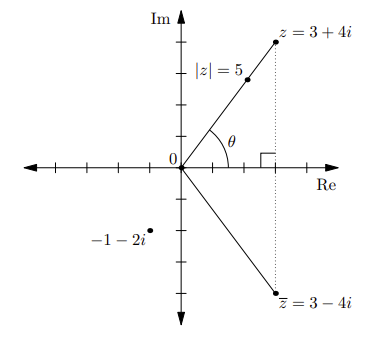
\includegraphics[width=0.5\linewidth]{complex_numbers.png}
\caption{An illustration of complex numbers (Credit: Evan Chen).}
\end{figure}
\end{center}

A consequence of this is that if \[z = re^{i\theta} = r\cis(\theta)\] then \[\ol{z} = re^{-i\theta} = r\cis(-\theta).\]

\begin{theorem*}[De Moivre's Theorem]
In general, \[\cis(\theta)^n = \cis(n\theta)\] for any integer $n$.
\end{theorem*}
\begin{proof}
Notice that \[\cis(\theta)^n = \left(e^{i\theta}\right)^n = e^{i(n\theta)} = \cis(n\theta)\] as required.
\end{proof}

This representation is especially useful for working with powers and roots of complex numbers, and although some of these won't be used immediately in this handout, they will become very useful in the future.

\newpage

\section{Roots and the Fundamental Theorem of Algebra}

We can now introduce the indispensable concept of a root.

\begin{definition*}[Root]
For a polynomial $P(x)$, we say that $r$ is a root of $P(x)$ if and only if $P(r) = 0$. Importantly, $r$ can be a complex number.
\end{definition*}

We can give some examples of this as well.

\begin{example*}
\begin{itemize}
\item The roots of the polynomial $P(x) = x^2-1$ are $x = 1$ and $x = -1$, since $P(1) = 0$ and $P(-1) = 0$.
\item The root of the polynomial $P(x) = x+2$ is $x = -2$, since $P(-2) = 0$.
\item The roots of the polynomial $P(x) = x^3+6x^2+11x+6$ are $x = -1$, $x = -2$, and $x = -3$, since $P(-1) = P(-2) = P(-3) = 0$.
\end{itemize}
\end{example*}

Now, in order to build up to the Fundamental Theorem of Algebra, we need to establish a few items; to study roots more effectively, we need ways for manipulating polynomials.

Just like how we can do arithmetic with numbers, we can also do arithmetic with polynomials. If we have two polynomials $P(x) = a_nx^n+a_{n-1}x^{n-1}+\cdots+a_0$ and $Q(x) = b_nx^n+b_{n-1}x^{n-1}+\cdots+b_0$, then we say that:

\begin{align*}
P(x)+Q(x) &= (a_n+b_n)x^n+(a_{n-1}+b_{n-1})x^{n-1}+\cdots+(a_0+b_0) \\
P(x)-Q(x) &= (a_n-b_n)x^n+(a_{n-1}-b_{n-1})x^{n-1}+\cdots+(a_0-b_0)
\end{align*}

which behaves exactly as you would expect. If the degrees are not equal, simply match degrees and sum the coefficients of the two polynomials.

\subsection{Polynomial Multiplication and Long Division}

We can also develop the notion of polynomial multiplication and division. Multiplication is rather straightforward:

\begin{definition*}[Polynomial Multiplication]
To multiply two polynomials $P(x)$ and $Q(x)$, we distribute the terms of $P(x)$ onto $Q(x)$ and combine like terms.
\end{definition*}

For instance,

\begin{example*}
Multiply the polynomials $x+3$ and $x^2+4x+5$.
\end{example*}

We write that \[(x+3)(x^2+4x+5) = x(x^2+4x+5)+3(x^2+4x+5)\] using the distributive property. Then, \[x(x^2+4x+5)+3(x^2+4x+5) = (x^3+4x^2+5x)+(3x^2+12x+15)\] by multiplying the two polynomials in each term. Finally, this equates to \[x^3+(4x^2+3x^2)+(5x+12x)+15 = x^3+7x^2+17x+15.\]

\begin{example*}
Multiply the two polynomials $x^2+x+1$ and $x^2-5x+3$.
\end{example*}

We perform the same method:

\begin{align*}
(x^2+x+1)(x^2-5x+3) &= x^2(x^2-5x+3)+x(x^2-5x+3)+1(x^2-5x+3) \\
&= (x^4-5x^3+3x^2)+(x^3-5x^2+3x)+(x^2-5x+3) \\
&= x^4+(-5+1)x^3+(3-5+1)x^2+(3-5)x+3 \\
&= x^4-4x^3-x^2-2x+3.
\end{align*}

We can also divide two polynomials using polynomial long division. Similarly to how we can divide two numbers by getting rid of the leftmost digit everytime:

\begin{center}
\longdivision[0]{12345}{13}
\end{center}

we can do the same for polynomial long division. The key things that we must notice is that:

\begin{itemize}
\item After every line, we find the largest multiple of $13$ that is at most the number we are trying to subtract off of.
\item The answer/quotient remains on the top while the remainder is the final remaining number.
\item We always bring down the next number after finished subtracting the multiple of $13$.
\end{itemize}

Keeping these in mind, we can develop an analogous method for polynomial long division.

\begin{example*}
Divide the polynomial $x^3+2x^2+1$ by $x+3$.
\end{example*}

We start by writing out the division chart:

\begin{center}
\polylongdiv[stage=0]{x^3+2x^2+1}{x+3}
\end{center}

ensuring that any terms with a coefficient of $0$ are also taken into account, and have a space (in this case, $0x$). Next, since we are aiming to get rid of the $x^3$, we multiply $x+3$ by $x^2$ and subtract to get:

\begin{center}
\polylongdiv[stage=4]{x^3+2x^2+1}{x+3}
\end{center}

Next, we wish to get rid of the $-x^2$, so we can multiply $x+3$ by $-x$ and subtract from $-x^2$ to get:

\begin{center}
\polylongdiv[stage=7]{x^3+2x^2+1}{x+3}
\end{center}

where we have already brought down the $1$. Finally, we want to get rid of the $3x$, which can be done by multiplying $x+3$ by $3$ and subtracting:

\begin{center}
\polylongdiv[stage=10]{x^3+2x^2+1}{x+3}
\end{center}

giving an quotient of $x^2-x+3$ and a remainder of $-8$. This process is relatively straight forward, so we present one more example.

\begin{example*}
Divide $x^3+2x^2-x+5$ by $x^2-2$.
\end{example*}

We start by writing out the chart:

\begin{center}
\polylongdiv[stage=0]{x^3+2x^2-x+5}{x^2-2}
\end{center}

Wishing to get rid of the $x^3$ term, we can multiply $x^2-2$ by $x$, subtract, and bring down the $5$ to get:

\begin{center}
\polylongdiv[stage=4]{x^3+2x^2-x+5}{x^2-2}
\end{center}

Now, we want to get rid of the $2x^2$, so we can multiply $x^2-2$ by $2$ and subtract to finish:

\begin{center}
\polylongdiv[stage=8]{x^3+2x^2-x+5}{x^2-2}
\end{center}

resulting in a quotient of $x+2$ and a remainder of $x+9$.

After you feel comfortable with this, we can move onto the quotient-remainder form.

\subsection{Quotient-Remainder Form}

Just as we can divide two numbers and get a result (quotient) as well as a remainder, we can do the same for polynomials. For example, if I were to divide $14$ by $3$, I could write that \[14 = 4\cdot 3+2\] where $4$ is the quotient and $2$ is the remainder. Notice that I can't write that $14 = 3\cdot 3 + 5$, since $14$ hasn't been fully divided by $3$. We can establish a similar result with polynomials (building off the previous section).

\begin{lemma*}[Quotient-Remainder Form]
If we have two polynomials $P(x)$ and $D(x)$, we can write that \[P(x) = Q(x)D(x)+R(x)\] where $Q(x)$ is the quotient when we divide $P$ by $D$ and $R(x)$ is the remainder when we divide $P$ by $D$. We also have the condition that $\deg R < \deg D$, since if this was not true, then $P$ hasn't been fully divided by $D$.
\end{lemma*}

We can also establish a key word relating to this:

\begin{definition*}[Divides]
We say that a polynomial $D(x)$ divides $P(x)$ if and only if there is no remainder ($R(x) = 0$) when we divide $P$ by $D$.
\end{definition*}

This is similar to how we say that $3$ divides $6$, since when we divide the two, there is no remainder.

We now can establish a very important theorem.

\begin{theorem*}[The Factor Theorem]
If $r$ is a root of a polynomial $P(x)$, then $x-r$ divides the polynomial $P$.
\end{theorem*}
\begin{proof}
Now, consider when we divide a polynomial $P(x)$ by a linear polynomial $D(x) = x-r$. Then, we get that \[P(x) = Q(x)(x-r)+R(x).\] If we let $r$ be a root of $P$, then we know that $P(r) = 0$, so \[0 = P(r) = Q(r)(r-r)+R(r) = R(r).\] Now, since $\deg R < \deg D$, we know that we must have that $\deg R = 0$. In other words, $R$ must be a constant, and we just saw that it is equal to $0$. Thus, we get that $x-r$ divides $P(x)$.
\end{proof}

Thus, if a polynomial $P$ has roots $r_1$, $r_2$, $\dots$, $r_n$ (counted with multiplicity, which we define next), we know that \[P(x) = c(x-r_1)(x-r_2)\cdots(x-r_n)\] for some constant $c$, because the factor theorem says that $x-r_1$, $x-r_2$, $\dots$, $x-r_n$ all must divide the polynomial, so $P$ must be a multiple of all of them. Hence, intuitively, a degree $n$ polynomial has at most $n$ real roots.

We now give a few examples to illustrate the idea.

\begin{example*}
Divide the polynomial $P(x) = x^4+x^2-1$ by the polynomial $D(x) = x^2-2x+1$ and express the answer in Quotient-Remainder form.
\end{example*}

We can divide the two polynomials using polynomial long division, and get that \[x^4+x^2-1 = (x^2+2x+4)(x^2-2x+1)+(6x-5)\] which is the required form.

\begin{example*}
Find the polynomial with smallest degree whose roots are $1$, $2$, and $3$.
\end{example*}

Since the roots are $1$, $2$, and $3$, we know that the polynomial must have the factors $x-1$, $x-2$, and $x-3$. Thus, the smallest polynomial would be \[P(x) = (x-1)(x-2)(x-3) = x^3-6x^2+11x-6.\]

\subsection{The Fundamental Theorem of Algebra}

We now want to answer the question of how many roots a general polynomial will have. This is where the Fundamental Theorem of Algebra comes into play.

We first define the idea of multiplicity.

\begin{definition}[Multiplicity]
A root $r$ of a polynomial $P$ has multiplicity $k$ if $k$ is the largest integer such that $(x-r)^k$ divides $P$. \footnote{Alternatively, a root $r$ has multiplicity $k$ if \[P(r) = P'(r) = \cdots = P^{(k-1)}(r) = 0\] and $P^k(r) \neq 0$.}
\end{definition}

\begin{theorem}[The Fundamental Theorem of Algebra]
Every nonzero univariate polynomial $P$ with complex coefficients has, counted with multiplicity, exactly $\deg P$ complex roots.
\end{theorem}

We say ``counted with multiplicity'' because any roots that have multiplicity $2$ are counted twice, multiplicity $3$ counted thrice, and so on. We won't prove this theorem here because it is very involved, but we can still reap the rewards.

What this tells us is that for any polynomial $P$, once we find $\deg P$ complex roots, we know that these are all the roots and don't have to look for more.

\begin{example*}
Compute the multiplicity of the root $x = 1$ in the polynomial $x^3-4x^2+5x-2$.
\end{example*}

We can see that $1$ is a root of this polynomial so we can divide the polynomial by $x-1$ to get the quotient of $x^2-3x+2$. Now, we can see that $1$ is still a root of this, so we can divide by $x-1$ again to $x-2$. Clearly, $x = 1$ is not a root of this, so $x-1$ divides the original polynomial twice, implying that $1$ has multiplicity $2$.

\begin{example*}
Use the Fundamental Theorem of Algebra to find all the roots of $x^3-2x^2+x$.
\end{example*}

We can see that $x = 0$ is a root, and $x = 1$ is a root with multiplicity $2$. By the Fundamental Theorem of Algebra, there must be $3$ roots, and we have found all of them (since $1+2 = 3$).

\subsection{Root Finding Methods and Conjugates}

Now that we know how many roots a given polynomial must have, we want to have some ways of finding these roots. Unfortunately, this gets increasingly difficult as the degree of the polynomial increases, however there are some things we can take advantage of. These include the:

\begin{itemize}
\item The Quadratic Formula
\item Conjugate Theorem
\item Rational Root Theorem
\item The Intermediate Value Theorem
\item Newton's Method.
\end{itemize}

\subsubsection{The Quadratic Formula}

We will not spend much time here, and instead encourage the reader to learn this themselves, however we provide the main idea here.

\begin{theorem*}[Quadratic Formula]
For a polynomial $P(x) = ax^2+bx+c$, it has roots \[\dfrac{-b\pm\sqrt{b^2-4ac}}{2a}.\]
\end{theorem*}
\begin{proof}
Suppose we have the quadratic \[ax^2+bx+c = 0\] and wish to find all $x$ satisfying this. Then, we can divide both sides by $a$ to get that \[x^2+\dfrac{b}{a}x+\dfrac{c}{a} = 0.\] Now, adding $\tfrac{b^2}{4a^2}$ to both sides, we get that \[\left(x^2+\dfrac{2b}{2a}x+\dfrac{b^2}{4a^2}\right)+\dfrac{c}{a} = \left(x+\dfrac{b}{2a}\right)^2+\dfrac{c}{a} = \dfrac{b^2}{4a^2}.\] Subtracting $\tfrac{c}{a}$ from both sides and square rooting, we get \[x+\dfrac{b}{2a} = \dfrac{\pm\sqrt{b^2-4ac}}{2a}\] and isolating $x$ gives the desired conclusion.
\end{proof}

We can follow this with an example.

\begin{example*}
Compute the roots of $x^2-4x+7$.
\end{example*}

By the quadratic formula, we get that the roots are \[\dfrac{4\pm\sqrt{-12}}{2} = 2\pm i\sqrt{3}.\]

\subsubsection{Conjugate Theorem}

We can start off by defining the idea of a conjugate.

\begin{definition*}[Conjugate]
The conjugate of a number of the form $a+b\sqrt{d}$ for real numbers $a$, $b$, $d$ is $a-b\sqrt{d}$. Similarly, the conjugate of a number of the form $a+bi$ for real numbers $a$, $b$ is $a-bi$.
\end{definition*}

We denote the conjugate of a number $a$ to be $\ol{a}$. We can also find some properties to do with conjugates.

\begin{lemma*}[Conjugate properties]
In the following examples, let $a$ and $b$ be arbitrary variables (complex or real). Then,
\begin{itemize}
\item $\ol{a+b} = \ol{a}+\ol{b}$
\item $\ol{a-b} = \ol{a}-\ol{b}$
\item $\ol{a\cdot b} = \ol{a}\cdot\ol{b}$
\item $\ol{a^n} = \ol{a}^n$
\item $\ol{a\div b} = \ol{a}\div \ol{b}$.
\end{itemize}
\end{lemma*}

In other words, conjugates distribute over arithmetic. We encourage the reader to verify all of these properties (try substituting $a = x+yi$, and $b =w+zi$ into the properties and proving them).

So why should we care? It turns out that for a polynomial with real coefficients, we can make a very useful statement about roots and their conjugates.

\begin{theorem*}[Complex Conjugate Root Theorem]
If a real polynomial $P(x)$ has a complex root $r$, then $\ol{r}$ is also a root of $P$.
\end{theorem*}
\begin{proof}
Let $r$ be a root of $P(x)$. Then, if we let \[P(x) = a_nx^n+a_{n-1}x^{n-1}+\cdots+a_0\] we know that: \[0 = P(r) = a_nr^n+a_{n-1}r^{n-1}+\cdots+a_0.\] Taking the conjugate of both sides, we have that:
\begin{align*}
0 &= \ol{a_nr^n+a_{n-1}r^{n-1}+\cdots+a_0} \\
&= \ol{a_nr^n}+\ol{a_{n-1}r^{n-1}}+\cdots+\ol{a_0} \\
&= \ol{a_n}\ol{r^n}+\ol{a_{n-1}}\ol{r^{n-1}}+\cdots+\ol{a_0}.
\end{align*}
Now, since the coefficients $a_k$ are real numbers, we know that the conjugate does not change their value. Hence,
\begin{align*}
0 &= \ol{a_n}\ol{r^n}+\ol{a_{n-1}}\ol{r^{n-1}}+\cdots+\ol{a_0} \\
&= a_n\ol{r^n}+a_{n-1}\ol{r^{n-1}}+\cdots+a_0 \\
&= a_n\ol{r}^n+a_{n-1}\ol{r}^{n-1}+\cdots+a_0
\end{align*}
so $\ol{r}$ is also a root as required.
\end{proof}

There is also an analogous version for the irrational conjugate.

\begin{theorem*}[Irrational Conjugate Root Theorem]
If a rational polynomial $P(x)$ has a real root of the form $a+b\sqrt{d}$ for real numbers $a$, $b$, and $d$, then $a-b\sqrt{d}$ is also a root of $P$.
\end{theorem*}

We omit the proof here but encourage the reader to try it themselves (it is very similar to the complex conjugate proof). We say that a polynomial is rational if all its coefficients are rational.

We provide one example.

\begin{example*}
A monic rational polynomial $P$ has roots $2+3i$, $1-\sqrt{2}$. Compute the minimum degree of $P$ and the corresponding value of $P$.
\end{example*}

Since the coefficients are rational (hence real), the polynomial is a real polynomial. Thus, applying the Complex Conjugate Root Theorem, we know that $2-3i$ must also be a root. In addition, by the Irrational Conjugate Root Theorem, $1+\sqrt{2}$ is also a root. Hence, we try the polynomial: \[P = (x-(2+3i))(x-(2-3i))(x-(1+\sqrt{2}))(x-(1-\sqrt{2}))\] which expands nicely into \[P = x^4 - 6 x^3 + 20 x^2 - 22 x - 13\] which is of degree $4$, as required.

This concludes our analysis of conjugates.

\begin{remark*}
There is a lot more to the subject, but it is under the name ``algebraic number theory'' and requires quite a lot of background that we have not developed here. If the reader is curious, feel free to look it up and explore!
\end{remark*}

\subsubsection{Rational Root Theorem}

A lot of times, we want to restrict our attention to rational roots and not worry about irrational roots. In that case, if we are dealing with an integer polynomial (a polynomial with integer coefficients), we have a very useful statement about these roots.

\begin{theorem*}[Rational Root Theorem]
For a polynomial \[P(x) = a_nx^n+a_{n-1}x^{n-1}+\cdots+a_0\] if there is a rational root $r = \pm\tfrac{p}{q}$, where $\gcd(p, q) = 1$ such that $P(r) = 0$, then it must be the case that:
\begin{itemize}
\item $p$ divides $a_0$ (in other words, $p$ is a factor of $a_0$)
\item $q$ divides $a_n$ ($q$ is a factor of $a_n$).
\end{itemize}
\end{theorem*}

The proof of this involves modular arithmetic, so feel free to skip it if you aren't comfortable with this yet.

\begin{proof}
Notice that we have \[a_np^n\left(q^{-1}\right)^n+a_{n-1}p^{n-1}\left(q^{-1}\right)^{n-1}+\cdots+a_0 = 0\] so multiplying by $q^n$, we get that \[a_np^n+a_{n-1}p^{n-1}q+\cdots+a_0q^n = 0.\] Taking this equation modulo $p$, the equation simplifies to just \[a_0 \equiv 0 \pmod{p}\] so $p \mid a_0$. Doing the same for $q$, we obtain that $q$ divides $a_n$, so we finish.
\end{proof}

This is an extremely useful fact, and is often used to find roots. We now present an example.

\begin{example*}
Find all the roots of $12x^3 - 16x^2 + 7x - 1$.
\end{example*}

By the rational root theorem, the possible roots are: \[x \in \{\pm\tfrac{1}{1}, \pm\tfrac{1}{2}, \pm\tfrac{1}{3}, \pm\tfrac{1}{4}, \pm\tfrac{1}{6}, \pm\tfrac{1}{12}\}\] and their negatives. Trying all of these values, we see that $\tfrac{1}{2}$ works, so dividing the polynomial by $x-\tfrac{1}{2}$ gives $12 x^2 - 10 x + 2$, which has roots $\tfrac{1}{2}$ and $\tfrac{1}{3}$. Thus, the answer is $\tfrac{1}{2}$ with multiplicity $2$ and $\tfrac{1}{3}$.

It is worth noting that \[12x^3-16x^2+7x-1 \neq \left(x-\tfrac{1}{2}\right)^2\left(x-\tfrac{1}{3}\right)\] since we need a multiplicative factor to match the coefficients, not just the roots. We actually have \[12x^3-16x^2+7x-1 = 12\left(x-\tfrac{1}{2}\right)^2\left(x-\tfrac{1}{3}\right) = (2x-1)^2(3x-1).\]

\subsubsection{The Intermediate Value Theorem}

The following theorem is very intuitive. Say that we have a polynomial $P(x)$. Then, because it is continuous, over any interval, it must achieve all of the values between the endpoints.

\begin{theorem*}[The Intermediate Value Theorem]
For any polynomial $P(x)$, let $[a, b]$ be an interval. Then, for any $c$ satisfying $P(a) \le c \le P(b)$, there exists $c'$ where $c' \in [a, b]$ such that $P(c') = c$.
\end{theorem*}

Just to be clear $\in$ is read as ``in'', so in the previous theorem, this means that $c'$ is in the interval $[a, b]$.

A corollary of this is that if we have a value $a$ and $b$ where $P(a)$ is negative and $P(b)$ is positive, then there must exist a root somewhere between $a$ and $b$.

This becomes most intuitive if we look at a graph of a polynomial. Then, we can see that it must pass through all the $y$-values between $f(a)$ and $f(b)$ at some point, which is essentially the theorem above.

Just to ensure that this is internalized, try to draw a continuous graph that passes through $(0, 1)$ and $(2, 3)$ without ever touching the line $y = 2$. It's impossible right?! The main point is that since the graph is continuous, we cannot have any gaps, and so the theorem follows.

At this point, it is worth noting that we are assuming that polynomials are continuous functions (which they are), without proof, because the proof of this is not relevant at this point, and would just distract us from the goal at hand.

We now give an example of this.

\begin{example*}
Find an interval $[a, b]$ such that $|b-a| \le 0.5$ and there exists a root $r$ of the polynomial $P(x) = x^3-2x^2+3x+5$ in this interval.
\end{example*}

We start by finding $P(-1) = -1$ and $P(0) = 5$. Thus, there must exist a root in the range $[-1, 0]$. We can also find $P\left(-\tfrac{1}{2}\right) = \tfrac{23}{8}$ to get that it must be in the interval $[-1, -\tfrac{1}{2}]$, and this range is small enough, as required.

\begin{remark*}
The actual root is $r \approx -0.89456$.
\end{remark*}

\subsubsection{Newton's Method}

\textbf{This section is not required.}

If you are not comfortable with the ideas above, please understand them before proceeding. On the other hand, if you do not know basic calculus (namely differentiation), you should either learn it (preferably), or skip this section; it is not necessary for competitions, but is pretty interesting.

With that disclaimer, we can proceed!

Newton's method is a root finding algorithm that iteratively generates better and better estimates for the location of the root of a polynomial.

\begin{center}
\begin{figure}[h!]
\centering
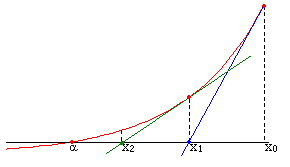
\includegraphics[width=0.5\linewidth]{newtons_method.png}
\caption{An illustration of Newton's method.}
\end{figure}
\end{center}

The idea is to select an initial guess $x_0$ for the location of the root. The closer it is, the better chance the method will find the correct location, and won't diverge to infinity. Next, we compute where the tangent at that point intersects the $x$-axis, and lets that be the next term, $x_1$. Repeating this many times will give $x_i$ that get closer and closer to the true value of the root.

We now formalize this idea. The slope of the line tangent to $P(x)$ at the point $x = x_0$ is $P'(x_0)$, by definition. Thus, using point-slope form, we can find the equation of the line through $(x_0, P(x_0))$ to be \[y - P(x_0) = P'(x_0)(x - x_0).\] Now, the point at which this intersects the $x$-axis is $(x_1, 0)$, so solving for $x$, we get that \[x_1 = x_0-\dfrac{P(x_0)}{P'(x_0)}.\] Repeating this gives us the required result:

\begin{theorem*}[Newton's Method]
Let $x_0$ be a real number. Then, the sequence of numbers $x_1$, $x_2$, $\dots$ defined by \[x_{i+1} = x_i-\dfrac{P(x_i)}{P'(x_i)}\] for integers $i \ge 0$ either diverges or approaches the value of a root.
\end{theorem*}

This is very useful for computers, since we can use this algorithm to get a numerical approximation for the location of a root.

With this, we conclude our analysis of roots and root finding methods.

\subsection{Exercises}

\begin{problem}[1]{}
What is the quotient and remainder when we divide the polynomial $x^5+2x^4+3x^3+4x^2+5x+6$ by $x+1$?
\end{problem}
\begin{problem}[2]{}
What is the quotient and remainder when we divide the polynomial $3x^3+4x^2+5x+6$ by $x^2+2$?
\end{problem}
\begin{problem}[3]{}
What are the polynomials of smallest degree with roots $1$, $i$, $-1$, and $-i$?
\end{problem}
\begin{problem}[4]{}
What is the multiplicity of the root $r = 1$ in the polynomial $x^3-3x^2+3x-1$?
\end{problem}
\begin{problem}[5]{}
How many roots does the polynomial $x^5-100x^4-1$ have?
\end{problem}
\begin{problem}[6]{}
Some problems on root finding:
\begin{enumerate}
\item Compute the roots of $x^2-x-1 = 0$.
\item Given that $1-\sqrt{2}$ and $2-\sqrt{3}$ are the roots of a rational monic polynomial of minimal degree, find this polynomial.
\item Given that $1$ and $i$ are the roots of a real monic polynomial of minimal degree, find this polynomial.
\item Approximate a real root of $3x^3-5x^2+x+5$ in an interval of size at most $0.5$. How do you know it's the only real root?
\item Show that it is impossible for a real polynomial $P$ to have exactly $\deg P - 1$ real roots.
\end{enumerate}
\end{problem}

\newpage

\section{Symmetric Polynomials and Vieta's Formulae}

We now move onto some problems that have to do with computations pertaining to roots. We first define the idea of a symmetric polynomial.

\begin{definition*}[Symmetric Polynomial]
A symmetric polynomial is a polynomial which remains unchanged if its variables are permuted.
\end{definition*}

This is most easily understood with a few examples.

\begin{example*}
\begin{itemize}
\item The polynomial $x_1^2+x_2^2+x_3^2$ is a symmetric polynomial because no matter how we permute the variables, the polynomial doesn't change. More concretely,
\begin{align*}
x_1^2+x_3^2+x_2^2 \\
x_2^2+x_1^2+x_3^2 \\
x_2^2+x_3^2+x_1^2 \\
x_3^2+x_1^2+x_2^2 \\
x_3^2+x_2^2+x_1^2
\end{align*}
are all still equal to the original polynomial, since we are effectively just moving around the terms.
\item The polynomial $2x_1^2+x_2^3+x_3^2$ is not a symmetric polynomial, since if I swap $x_1$ and $x_2$, it creates a completely different polynomial.
\end{itemize}
\end{example*}

We can now get to the main idea of why symmetric polynomials are useful.

\begin{definition*}[Elementary Symmetric Polynomial]
An elementary symmetric polynomial $e_k$ of $n$ variables is ``equal'' to summing the $n$ variables $k$ at a time.
\end{definition*}

It is worth noting that this is not the real definition, but is certainly easier to digest.

\begin{example*}
\begin{itemize}
\item The polynomial $x_1x_2+x_1x_3+x_2x_3$ is the $2$nd elementary symmetric polynomial for $3$ variables, since it takes the sum of the products of all the possible pairs (which is why we say ``$2$ at a time'') of variables.
\item The polynomial $x_1x_2x_3+x_1x_2x_4+x_1x_3x_4+x_2x_3x_4$ is the $3$rd elementary symmetric polynomial for $4$ variables, since it takes the sum of all the distinct products of triplets possible.
\item The polynomial $x_1x_2+x_1x_3+x_1x_4+x_2x_3+x_2x_4+x_3x_4$ is the $2$nd elementary symmetric polynomial for $4$ variables, since it takes the sum of all the distinct products of pairs possible.
\item The polynomial $x_1x_2x_3$ is the $3$rd elementary symmetric polynomial for $3$ variables, since it takes the ``sum'' of all the distinct products of triplets possible.
\item The polynomial $x_1+x_2+x_3$ is the $1$st elementary symmetric polynomial for $3$ variables, because it takes the sum of all the distinct products of singular elements (meaning sum of all the elements).
\end{itemize}
\end{example*}

It is also worth noting that we denote the $k$th symmetric polynomial with $n$ variables as $e_k\left(x_1, x_2, \dots, x_n\right)$ for variables $x_1$, $x_2$, $\dots$, $x_n$. We also have the shorthand $e_k(n)$ if we know what the variables are.

Now, there is a very useful fact that follows from the definition of the symmetric polynomial. To see what it is, let's do a quick exercise. If a polynomial $P(x)$ has two roots $r_1$, $r_2$, what is the polynomial $P$ explicitly?

Well, we know that \[P(x) = (x-r_1)(x-r_2) = x^2-(r_1+r_2)x+r_1r_2 = x^2-e_1(r_1, r_2)x+e_2(r_1, r_2)\] where we group by the degree of $x$.

Now, we ask the same question, but for a polynomial with roots $r_1$, $r_2$, and $r_3$. Then,

\begin{align*}
P(x) &= (x-r_1)(x-r_2)(x-r_3) \\
&= x^3-(r_1+r_2+r_3)x^2+(r_1r_2+r_1r_3+r_2r_3)x-r_1r_2r_3 \\
&= x^3-e_1(r_1, r_2, r_3)x^2+e_2(r_1, r_2, r_3)x-e_3(r_1, r_2, r_3).
\end{align*}

Finally, we do this for a polynomial with roots $r_1$, $r_2$, $r_3$, and $r_4$. Then,

\begin{align*}
P(x) &= (x-r_1)(x-r_2)(x-r_3)(x-r_4) \\
&= x^4-(r_1+r_2+r_3+r_4)x^3+(r_1r_2+r_1r_3+r_1r_4+r_2r_3+r_2r_4+r_3r_4)x^2 \\
&\phantom{=} -(r_1r_2r_3+r_1r_2r_4+r_1r_3r_4+r_2r_3r_4)x+r_1r_2r_3r_4 \\
&= x^4-e_1(4)x^3+e_2(4)x^2-e_3(4)x+e_4(4).
\end{align*}

By now, we hope that the reader has recognized the pattern. Our results can be encapsulated in the following theorem.

\begin{theorem*}[Vieta's Formulae]
If a polynomial \[P(x) = a_nx^n+a_{n-1}x^{n-1}+\cdots+a_0\] is such that $\deg P = n$, and has roots $r_1$, $r_2$, $\dots$, $r_n$. Then, in general, \[e_k(r_1, r_2, \cdots, r_n) = (-1)^k\cdot \dfrac{a_{n-k}}{a_n}.\] Notably, if the polynomial is monic, then the RHS is just equal to $(-1)^k\cdot a_{n-k}$.
\end{theorem*}

It is very important that the $-$ sign isn't forgotten. An easy way to remember this is that we assign the leading term a sign of $+$, and alternate for each term after it ($-$, $+$, $-$, etc.) until the final term, ensuring that any terms with coefficient $0$ are also counted. Then, when using the theorem, we simply multiply the coefficient by the corresponding sign.

It is worth doing an example to demonstrate this theorem.

\begin{example*}
A polynomial $P(x) = 2x^3-6x^2+5x-4$ has roots $r_1$, $r_2$, and $r_3$. Compute $e_1(3)$, $e_2(3)$, and $e_3(3)$.
\end{example*}

This is just a direct application of the theorem. We know that \[e_1(3) = r_1+r_2+r_3 = (-1)^1\cdot \dfrac{-6}{2} = 3\] by applying the theorem. Similarly, \[e_2(3) = r_1r_2+r_1r_3+r_2r_3 = (-1)^2\cdot \dfrac{5}{2} = \dfrac{5}{2}\] and \[e_3(3) = r_1r_2r_3 = (-1)^3\cdot \dfrac{-4}{2} = 2\] which finishes the example.

The best thing about this theorem is that we never needed to compute the roots to figure out what the elementary symmetric polynomials evaluate to: they just come directly from the theorem.

However, the question is ``why should we care''. After all, this is only applicable in a certain case: when the expression we want to evaluate is an elementary symmetric polynomial. The chance that this actually happens is rather small. However, one other theorem broadens our scope significantly.

\begin{theorem*}[Fundamental Theorem of Symmetric Polynomials]
Any symmetric polynomial can be expressed as a polynomial in elementary symmetric polynomials.
\end{theorem*}

A corollary of this is that any symmetric polynomial (like $r_1^2+r_2^2+r_3^2$) can be rewritten so that it can be evaluated solely using elementary symmetric polynomials.

\begin{example*}
\begin{itemize}
\item The polynomial $r_1^2+r_2^2+r_3^2 = (r_1+r_2+r_3)^2-2(r_1r_2+r_1r_3+r_2r_3) = e_1(3)^2-2e_2(3)$.
\item The polynomial $r_1^3+r_2^3+r_3^3 = (e_1(3))(e_1(3)^2-3e_2(3))+3e_3(3)$ (try expanding this!).
\item The non-polynomial (but rational function) $\tfrac{1}{r_1}+\tfrac{1}{r_2}+\tfrac{1}{r_3} = \tfrac{e_2(3)}{e_3(3)}$.
\end{itemize}
\end{example*}

This is extremely useful; now, we can compute many more expressions concerning roots, just from Vieta's formulae and elementary symmetric polynomials.

\subsection{Newton's Sums}

Now, we have the tools to compute arbitrary symmetric polynomials of the roots. However, one common theme that comes up a lot is wanting to find the sum of the $n$th powers of all the roots of a polynomial. For small $n$, this can be done easily:

For example, for a polynomial $P(x) = ax^3+bx^2+cx+d$ of degree $3$ with roots $r_1$, $r_2$, and $r_3$, let \[S_n = r_1^n+r_2^n+r_3^n.\] Then, computing $S_1$ is easy enough, it's just $-\tfrac{b}{a}$. For $S_2$, we have that \[S_2 = r_1^2+r_2^2+r_3^2 = (r_1+r_2+r_3)^2-2(r_1r_2+r_1r_3+r_2r_3) = \left(\dfrac{b}{a}\right)^2-2\left(\dfrac{c}{a}\right).\] Now, for $S_3$, we have to exert a little more effort:

\begin{align*}
S_3 &= r_1^3+r_2^3+r_3^3 \\
&= r_1^3+r_2^3+r_3^3-3r_1r_2r_3+3r_1r_2r_3 \\
&= (r_1+r_2+r_3)(r_1^2+r_2^2+r_3^2-(r_1r_2+r_1r_3+r_2r_3))+3r_1r_2r_3 \\
&= (r_1+r_2+r_3)((r_1+r_2+r_3)^2-3(r_1r_2+r_1r_3+r_2r_3))+3r_1r_2r_3
\end{align*}

where we use the factorization \[x^3+y^3+z^3-3xyz = (x+y+z)(x^2+y^2+z^2-xy-xz-yz).\] This can be computed from Vieta's formulae, but it isn't clear how we can proceed to even larger $n$, like $S_4$, and $S_5$. The answer to this question is Newton's Sums.

\begin{theorem*}[Newton's Sums]
For a polynomial $P(x)$ of degree $n$, if \[P(x) = a_nx^n+a_{n-1}x^{n-1}+\cdots+a_0\] and $P$ has roots $r_1$, $r_2$, $\cdots$, $r_n$, then \[a_nS_k+a_{n-1}S_{k-1}+\cdots+a_{n-k+1}S_1+k\cdot a_{n-k} = 0\] where we use the convention that $a_i = 0$ if $i < 0$.\footnote{Some authors like to add the initialization $S_0 = n$ as well.}
\end{theorem*}

Thus, we can calculate $S_k$ for an arbitrary $k$ recursively, by calculating $S_1$, $S_2$, and so on up until $S_k$. This is most clear with an example.

\begin{example*}
Let $P(x) = x^3+3x^2+4x-8$, and the roots be $r$, $s$, and $t$. Then, compute $r^4+s^4+t^4$.
\end{example*}

By Newton's Sums, we have that:

\begin{align*}
S_1+3 &= 0 \\
S_2+3S_1+8 &= 0 \\
S_3+3S_2+4S_1-24 &= 0 \\
S_4+3S_3+4S_2-8S_1 &= 0.
\end{align*}

By computing each variable using the first equation and substituting downward, we obtain $S_1 = -3$, $S_2 = 1$, $S_3 = 33$, and $S_4 = \boxed{-127}$, which is the desired answer.

\subsection{Exercises}


\begin{problem}[1]{}
Which of the following are symmetric polynomials?
\begin{enumerate}
\item $x+y$
\item $x^2+y^3$
\item $xy+xz+yz$
\item $x^2+y^2+z^2$
\item $x^y+x^z+y^x+y^z+z^x+z^y$
\end{enumerate}
\end{problem}
\begin{problem}[2]{}
Compute the $2$nd elementary symmetric polynomial for $5$ variables.
\end{problem}
\begin{problem}[3]{}
Let $P(x) = 2x^3-10x^2+5$, and let the roots be $r_1$, $r_2$, and $r_3$. Compute all of the elementary symmetric polynomials of the roots.
\end{problem}
\begin{problem}[4]{}
Let $P(x) = x^4-3x^3+x-10$. If it has roots $r_1$, $r_2$, $r_3$, and $r_4$, compute \[\dfrac{1}{r_1}+\dfrac{1}{r_2}+\dfrac{1}{r_3}+\dfrac{1}{r_4}.\]
\end{problem}
\begin{problem}[5]{}
Let the roots of the polynomial $x^3+2x^2+3x+4$ be $r$, $s$, and $t$. Compute the value of $(r+1)(s+1)(t+1)$.
\end{problem}
\begin{problem}[6]{}
This problem has two parts.
\begin{enumerate}
\item Express $x^2y+x^2z+xy^2+y^2z+xz^2+yz^2$ in a form that only uses elementary symmetric polynomials.
\item Let $r$, $s$, and $t$ be the roots of $P(x) = x^3+3x^2+6x+10$. Compute \[r^2s+r^2t+rs^2+s^2t+rt^2+st^2.\]
\end{enumerate}
\end{problem}
\begin{problem}[7]{}
\item Let $P(x) = x^{100}+3x+5$, and let it have roots $r_1$, $\cdots$, $r_{100}$. Compute \[r_1^{100}+r_2^{100}+\cdots+r_{100}^{100}.\]
\end{problem}
\begin{problem}[8]{}
Let $P(x) = x^4-x^3+x-3$. If it has roots $r_1$, $r_2$, $r_3$, and $r_4$, compute \[\dfrac{1}{1-r_1}+\dfrac{1}{1-r_2}+\dfrac{1}{1-r_3}+\dfrac{1}{1-r_4}.\]\footnote{For a hint, consider the quotient $\tfrac{P'(x)}{P(x)}$, after an application of the product rule.}
\end{problem}

\newpage

\section{Polynomial Construction}

This section will be about constructing a polynomial that satisfies a certain condition, which is a recurring theme that comes up a lot in contest problems. For example, you might be asked to find a polynomial that passes through some points, or has some specific roots, etc. This section deals with those tropes.

Now, before we start, it is worth stating the following theorem.

\begin{theorem*}[The Identity Theorem]
If two polynomials $P(x)$ and $Q(x)$ both of degree $n$ are equal at $n+1$, points then \[P(x) = Q(x).\]
\end{theorem*}

The reason that we state this is just a formality; it ensures that whenever we find a suitable polynomial, we know that it is the only such one satisfying the condition we want.

\subsection{Substitution and Transformations}

Suppose that we have a polynomial $P(x)$, with degree $n$, and roots $r_1$, $r_2$, $\dots$, $r_n$. Then, suppose we were asked to create a polynomial $Q(x)$ with roots $\alpha r_1$, $\alpha r_2$, $\dots$, $\alpha r_n$ for some scalar constant $\alpha$. We can then notice that \[Q(x) = c(x-\alpha r_1)(x-\alpha r_2)\cdots(x-\alpha r_n)\] for some constant $c$. Rewriting,

\begin{align*}
c(x-\alpha r_1)(x-\alpha r_2)\cdots(x-\alpha r_n) &= c\alpha^n\left(\dfrac{x}{\alpha}-r_1\right)\left(\dfrac{x}{\alpha}-r_2\right)\cdots\left(\dfrac{x}{\alpha}-r_n\right) \\
&= c\alpha^nP\left(\dfrac{x}{\alpha}\right).
\end{align*}

Thus, the polynomial with roots $\alpha r_1$, $\alpha r_2$, $\dots$, and $\alpha r_n$ is $P(x/\alpha)$, up to scaling.

However, this should make intuitive sense: if we plug in $\alpha r_k$ into this polynomial, then it is equal to $P(r_k)$, which is obviously $0$. Moreover, it seems that we have essentially transformed the original polynomial so that it has the roots that we want.

Applying a similar logic, say we wanted a polynomial with roots $2r_1+3$, $2r_2+3$, $\dots$, $2r_n+3$. Then, we want an expression such that when we substitute in one of these roots $2r_i+3$, it results in $r_i$. However, this expression is precisely $\tfrac{x-3}{2}$, so our required answer is just \[P\left(\dfrac{x-3}{2}\right)\] up to scaling. This demonstrates the power of this method: even without finding the roots, we are able to construct a new polynomial whose roots satisfy some property.

We give a concrete example.

\begin{example*}
The polynomial $P(x) = x^3-6x^2+11x-5$ has roots $r$, $s$, and $t$. Compute a polynomial with roots $2r-1$, $2s-1$, and $2t-1$.
\end{example*}

Reasoning through as before, we see that our desired polynomial is just $P\left(\tfrac{x+1}{2}\right)$. We multiply by $8$ to get rid of all fractions (note that this does not change the roots), so:

\begin{align*}
8P\left(\dfrac{x+1}{2}\right) &= 8\left(\dfrac{x+1}{2}\right)^3-48\left(\dfrac{x+1}{2}\right)^2+88\left(\dfrac{x+1}{2}\right)-40 \\
&= (x+1)^3-12(x+1)^2+44(x+1)-40 \\
&= x^3 - 9 x^2 + 23 x - 7
\end{align*}

as required.

\subsection{The Two-Polynomial Method}

This section has to do with when you are trying to find a polynomial that passes through some fixed points, and they fit some nice pattern or relationship.

This method is best demonstrated with examples, but just to get an idea of what lies ahead:

The idea of the Two-Polynomial Method is to construct a new polynomial that has many known roots, so that it can be factored explicitly. This then allows us to recover the original polynomial or evaluate it at new points.

\begin{example*}
Compute the degree $2009$ polynomial $P(x)$ that passes through the points $\left(k, \tfrac{1}{k}\right)$ for all integers $k = 1$, $2$, $\dots$, $2010$, and find $P(2011)$.
\end{example*}

It may be tempting to say that the answer is just $P(x) = \tfrac{1}{x}$ giving $\tfrac{1}{2011}$, however this isn't a polynomial! Hence, to solve this question, we need to use the Two-Polynomial Method.

To start, let's define a polynomial $Q(x)$ such that \[Q(x) = xP(x)-1.\] Then, notice that $Q(x)$ has roots at $x \in \{1, 2, \dots, 2010\}$, since for each of these values, \[Q(k) = kP(k)-1 = k\cdot \dfrac{1}{k}-1 = 0.\] Also, because $P$ has degree $2009$, $Q$ must have degree $2010$, implying that \[c(x-1)(x-2)\cdots(x-2010) = xP(x)-1\] for some constant $c$. Substituting $x = 0$ into this equation, we get that \[c(-1)^{2010}\cdot 2010! =c\cdot 2010! = -1\] so $c = -\tfrac{1}{2010!}$. Thus, all there is to verify is that \[P(x) = \dfrac{1}{x}\left(-\dfrac{(x-1)(x-2)\cdots(x-2010)}{2010!}+1\right)\] is a polynomial. Now, the constant term of the polynomial (in parenthesis) can be found by plugging in $x = 0$, and doing so gives a result of $0$. Thus, we can divide by $x$, implying that the RHS is a polynomial. This gives our required answer. To finish the problem, we compute:

\begin{align*}
P(2011) &= \dfrac{1}{2011}\left(-\dfrac{(2011-1)(2011-2)\cdots(2011-2010)}{2010!}+1\right) \\
&= \dfrac{1}{2011}\left(-\dfrac{2010!}{2010!}+1\right) \\
&= \boxed{0}.
\end{align*}

\begin{example*}[USAMO 1975/3]
A polynomial $P(x)$ of degree $n$ satisfies $P(k) = \tfrac{k}{k+1}$ for $k = 0$, $1$, $2$, $\dots$, $n$. Find $P(n + 1)$.
\end{example*}

We define an auxiliary polynomial $Q(x)$ such that \[Q(x) = (x+1)P(x)-x.\] Then, $Q(x)$ has degree $n+1$, and roots at $x = 0$, $1$, $\dots$, $n$. Hence, \[cx(x-1)(x-2)\cdots(x-n) = (x+1)P(x)-x\] for some constant $c$. Now, substituting $x = -1$, we get that \[c\cdot (n+1)!\cdot (-1)^{n+1} = 1\] implying that $c = \tfrac{(-1)^{n+1}}{(n+1)!}$. Therefore, \[P(x) = \dfrac{1}{x+1}\left(\dfrac{(-1)^{n+1}\cdot x(x-1)(x-2)\cdots(x-n)}{(n+1)!}+x\right)\] which we can check is indeed a polynomial. Finally,

\begin{align*}
P(n+1) &= \dfrac{1}{n+2}\left(\dfrac{(-1)^{n+1}(n+1)!}{(n+1)!}+n+1\right) \\
&= \boxed{\dfrac{(n+1)+(-1)^{n+1}}{n+2}}
\end{align*}

which is the desired result.

\subsection{Lagrange Interpolation}

So far, we have seen how to find a polynomial through some desired points, such as when we are given the roots of a polynomial, or a certain property that its points satisfy. Now, we generalize to finding a polynomial through any given points.

Suppose that we have $n$ points: $P_1$, $P_2$, $\dots$, $P_n$. Then, by the Identity Theorem, there is at most one polynomial of degree $n-1$ through these points. However, it turns out that there is exactly one such polynomial, and we can explicitly construct it. To do so, we use Lagrange Interpolation.

This is again best illustrated by example.

\begin{example*}
Find the unique cubic through the points $(-1, -15)$, $(0, -6)$, $(1, -3)$, and $(2, 6)$.
\end{example*}

Let this polynomial be $P(x)$. Consider the term $x(x-1)(x-2)$: clearly, this vanishes when $x = 0$, $x = 1$, or $x = 2$, but not at $x = -1$. Hence, we can scale this term to give the value we want at $x = -1$. In this case, if we take \[\tfrac{5}{2}x(x-1)(x-2)\] then it will give $0$ at $x \in \{0, 1, 2\}$, but $-15$ at $x = -1$. Now, if we create similar terms for each of the other points, then when we sum them all together and plug in a required point, all terms vanish except one, which gives the desired value.

Moreover, the polynomial with roots $-1$, $1$, and $2$ is $(x+1)(x-1)(x-2)$, and we scale this by $-3$ to make sure that at $x = 0$, it gives $-6$, giving
\[-3(x+1)(x-1)(x-2).\] Continuing, we get \[\tfrac{3}{2}(x+1)x(x-2)\] for the term corresponding to $(1, -3)$, and \[(x+1)x(x-1)\] for the term corresponding to $(2, 6)$.

Summing all of these together, we obtain \[P(x) = \tfrac{5}{2}x(x-1)(x-2)+ \tfrac{3}{2}(x+1)x(x-2)- 3(x+1)(x-1)(x-2)+ (x+1)x(x-1)\] which simplifies to \[P(x) = 2x^3 - 3x^2 + 4x - 6.\]

Now, notice that in the first expression for $P(x)$, when we plug in $x = -1$, the first term remains, however the remaining terms equal $0$, since they all have a factor of $x+1$. In addition, since the first term is scaled by the exact amount that we want, it will give the desired point! Similarly, if we plug in $x = 0$, $1$, or $2$, then only the corresponding term will remain, with the correct scaling as well.

\begin{example*}
Find the unique quadratic polynomial passing through the points $(0, 1)$, $(1, 3)$, and $(2, 7)$.
\end{example*}

Let the polynomial be $P(x)$. Then, $(x-1)(x-2)$ needs to be scaled by $\tfrac{1}{2}$ to give the point $(0, 1)$, the term $x(x-2)$ must be scaled by $-3$ to give $(1, 3)$, and $x(x-1)$ must be scaled by $\tfrac{7}{2}$ to give the point $(2, 7)$. Hence, the required polynomial is:

\begin{align*}
P(x) &= \tfrac{1}{2}(x-1)(x-2)-3x(x-2)+\tfrac{7}{2}x(x-1) \\
&= x^2+x+1
\end{align*}

which is the required answer.

This method is called Lagrange Interpolation. There also exists an explicit formula, although this is less commonly used in computational competitions (in contrast, it is used frequently in olympiads).

\begin{lemma*}[Lagrange Interpolation]
Suppose that there are $n$ points $P_i = (x_i, y_i)$, with all $x_i$ distinct, for $1 \le i \le n$. Then, \[P(x) = \sum_{i=1}^ny_i\prod_{j \neq i} \dfrac{x-x_j}{x_i-x_j}.\]
\end{lemma*}

Again, the formula is not the most important idea here; it is more beneficial for the reader to understand the underlying idea presented in the examples (it is more useful in proofs rather than computational problems, but we introduce it here).

\subsection{Finite Differences}

We conclude with the concept of Finite Differences. While it does not come up often, it's conceptually useful, since the methods used can be applied in many places.

We start by defining the forward difference operator for sequences.

\begin{definition*}[The Forward Difference for Sequences]
Given a sequence $a_0, a_1, a_2, \dots$, we define $\Delta$ applied to this sequence to produce a new sequence $\Delta a_0, \Delta a_1, \Delta a_2, \dots$, where \[\Delta a_n = a_{n+1} - a_n.\] In other words, $\Delta$ takes consecutive differences. We can then apply $\Delta$ again to this new sequence, giving $\Delta^2 a_n = \Delta(\Delta a_n)$, and so on. We call $\Delta^k a_n$ the $k$th forward difference of the sequence.
\end{definition*}

We now present an example that illustrates the use of forward differences.

\newpage

\begin{example*}
Consider the sequence $1, 4, 9, 16, 25, \dots$ of perfect squares. Applying $\Delta$ repeatedly gives the following difference table:

\begin{center}
\begin{tabular}{ccccccccc}
\hline
$1$ & & $4$ & & $9$ & & $16$ & & $25$ \\
\hline
& $3$ & & $5$ & & $7$ & & $9$ & \\
\hline
& & $2$ & & $2$ & & $2$ & & \\
\hline
\end{tabular}
\end{center}
where each row is obtained by taking consecutive differences of the row above.
\end{example*}

Notice that the second difference row is constant (equal to $2$). This suggests the following: a sequence is given by a polynomial of degree $n$ if and only if its $n$th difference row is constant (and nonzero). In the example above, the sequence $n^2$ is generated by a degree $2$ polynomial, consistent with the second difference row being constant.

We now extend this to polynomials.

\begin{definition*}[The Forward Difference]
For a polynomial $P(x)$, define the forward difference operator $\Delta$ to be: \[\Delta P(x) = P(x+1)-P(x).\]
\end{definition*}

This is consistent with the sequence definition, since applying $\Delta$ to the polynomial $P$ and evaluating at nonnegative integers gives exactly the sequence of differences $P(1)-P(0)$, $P(2)-P(1)$, $\dots$.

Also, this operator always decreases the degree of the polynomial by $1$, analogous to differentiation. We may also repeatedly apply the forward difference operator on a polynomial, similarly to a sequence.

Similarly to how we found that a sequence generated by a degree $n$ polynomial has its $n$th forward difference row equal to a non-zero constant, the analogous statement holds for polynomials:

\begin{theorem*}[The Forward Difference Theorem]
For a polynomial $P(x)$ of degree $n$ and leading coefficient $c$, the $n$th forward difference is constant and equal to $c\cdot n!$. In addition, all higher differences are zero (more explicitly, $\Delta^{n+1}P(x)=0$). 
\end{theorem*}

For example, in the example we gave, the polynomial $x^2$ has degree $2$ and leading coefficient $1$, so the $2$nd finite difference must be equal to $1\cdot 2! = 2$, which is consistent with our findings.

We illustrate this with an example that captures the essence of finite differences.

\begin{example*}
A cubic polynomial $P(x)$ has the property that $P(1) = 1$, $P(2) = 3$, $P(3) = 13$, and $P(4) = 37$. Compute $P(5)$.
\end{example*}

Notice that we could do this with Lagrange Interpolation, however it would be very inefficient and tedious. Thus, we rely on the Forward Difference Theorem. 

We compute the forward differences:

\begin{center}
\begin{tabular}{ccccccc}
\hline
$1$ & & $3$ & & $13$ & & $37$ \\
\hline
& $2$ & & $10$ & & $24$ & \\
\hline
& & $8$ & & $14$ & & \\
\hline
& & & $6$ & & & \\
\hline
\end{tabular}
\end{center}

Now, the key idea is that because it's a cubic polynomial, the third differences (the fourth row of the table) are constant. Thus, we can extend it by one, and backtrack to figure out $P(5)$.

\begin{center}
\begin{tabular}{ccccccccc}
\hline
$1$ & & $3$ & & $13$ & & $37$ & & $\textcolor{red}{81}$ \\
\hline
& $2$ & & $10$ & & $24$ & & $\textcolor{red}{44}$  &\\
\hline
& & $8$ & & $14$ & & $\textcolor{red}{20}$ & &\\
\hline
& & & $6$ & & $\textcolor{red}{6}$ & & &\\
\hline
\end{tabular}
\end{center}

Thus, the answer is $81$. In fact, a different little known fact is that if we take the left column ($1$, $2$, $8$, and $6$), then we can actually explicitly find the original polynomial by doing \[P(x) = 1\binom{x}{0}+2\binom{x}{1}+8\binom{x}{2}+6\binom{x}{3} = x^3+x^2+1.\] This result is called Newton's Forward Difference Formula.

\begin{theorem*}[Newton's Forward Difference Formula]
In general, for a polynomial $P(x)$ of degree $n$, \[P(x) = \sum_{k=0}^{\infty} (\Delta^kP)(0)\binom{x}{k}\] and since $\Delta^k P \equiv 0$ for $k \ge n+1$, the sum is finite.
\end{theorem*}

We won’t prove this explicitly, but it follows from repeated differences.

These results about finite differences are most useful when we are given a polynomial, as well as consecutive inputs values and their output values.

\newpage

\section{Problems}

\subsection{Easier Problems}

\begin{problem}[1]{AIME I 2018/1}
Let $S$ be the number of ordered pairs of integers $(a,b)$ with $1 \leq a \leq 100$ and $b \geq 0$ such that the polynomial $x^2+ax+b$ can be factored into the product of two (not necessarily distinct) linear factors with integer coefficients. Find the remainder when $S$ is divided by $1000$.
\end{problem}

\begin{problem}[2]{AIME I 2010/9}
Compute the maximum possible value of $a^3+b^3+c^3$ over all real numbers $(a, b, c)$ satisfying
\begin{align*}
a^3 &= abc+2 \\
b^3 &= abc+6 \\
c^3 &= abc+20.
\end{align*}
\end{problem}

\begin{problem}[3]{AIME II 2008/7}
Let $r$, $s$, and $t$ be the three roots of the equation \[8x^3+1001x+2008=0.\] Find $ (r+s)^3+(s+t)^3+(t+r)^3$.
\end{problem}

\begin{problem}[4]{Canada 1996}
If $\alpha$, $\beta$, and $\gamma$ are the roots of $x^3 - x - 1 = 0$, compute $\frac{1+\alpha}{1-\alpha} + \frac{1+\beta}{1-\beta} + \frac{1+\gamma}{1-\gamma}$.
\end{problem}

\begin{problem}[5]{AIME II 2020/11}
Let $P(x) = x^2 - 3x - 7$, and let $Q(x)$ and $R(x)$ be two quadratic polynomials also with the coefficient of $x^2$ equal to $1$. David computes each of the three sums $P + Q$, $P + R$, and $Q + R$ and is surprised to find that each pair of these sums has a common root, and these three common roots are distinct. If $Q(0) = 2$, then $R(0) = \dfrac mn$, where $m$ and $n$ are relatively prime positive integers. Find $m+n$.
\end{problem}

\begin{problem}[6]{USAMO 1984/1}
The product of two of the four roots of the quartic equation $x^4 - 18x^3 + kx^2+200x-1984=0$ is $-32$. Determine the value of $k$.
\end{problem}

\begin{problem}[7]{AIME II 2003/9}
Consider the polynomials $P(x) = x^6 - x^5 - x^3 - x^2 - x$ and $Q(x) = x^4 - x^3 - x^2 - 1.$ Given that $z_1$, $z_2$, $z_3$, and $z_4$ are the roots of $Q(x) = 0$, find $P(z_1) + P(z_2) + P(z_3) + P(z_4)$.
\end{problem}

\begin{problem}[8]{SMT Algebra 2013/9}
Let $a=-\sqrt{3}+\sqrt{5}+\sqrt{7},b=\sqrt{3}-\sqrt{5}+\sqrt{7},c=\sqrt{3}+\sqrt{5}-\sqrt{7}$. Evaluate \[\frac{a^4}{(a-b)(a-c)}+\frac{b^4}{(b-c)(b-a)}+\frac{c^4}{(c-a)(c-b)}.\]
\end{problem}

\begin{problem}[9]{MP4G 2025/11}
Solve for $a$:
\begin{eqnarray*}
a - b + c - d + e & = & 1 \\
a - 2b + 4c -8d + 16e & = & 128 \\
a - 3b + 9c - 27d + 81e & = & 2187 \\
a-4b+16c-64d+256e & = & 16384 \\
a-5b+25c-125d+625e & = & 78125.
\end{eqnarray*}
\end{problem}

\begin{problem}[10]{MP4G 2024/13}
Let $p$ be the unique polynomial of degree 6 such that \[p(n) = (-1)^n \binom{6}{n}\] for $n = 0$, $1$, $2$, $3$, $\dots$ , $6$. What is $p(7)$?
\end{problem}

\begin{problem}[11]{HMMT Algebra 2020/8}
Let $P(x)$ be the unique polynomial of degree at most $2020$ satisfying $P(k^2)=k$ for $k=0$, $1$, $2$, $\dots$, $2020$. Compute $P(2021^2)$.
\end{problem}

\begin{problem}[12]{HMMT Feb. Team 2015/1}
The complex numbers $x$, $y$, $z$ satisfy
\begin{align*}
xyz &= -4 \\
(x+1)(y+1)(z+1) &= 7 \\
(x+2)(y+2)(z+2) &= -3.
\end{align*}
Compute the value of $(x+3)(y+3)(z+3)$.
\end{problem}

\begin{problem}[13]{AIME I 2019/10}
For distinct complex numbers $z_1,z_2,\dots,z_{673}$, the polynomial \[ (x-z_1)^3(x-z_2)^3 \cdots (x-z_{673})^3 \]can be expressed as $x^{2019} + 20x^{2018} + 19x^{2017}+g(x)$, where $g(x)$ is a polynomial with complex coefficients and with degree at most $2016$. The value of \[ \left| \sum_{1 \le j <k \le 673} z_jz_k \right| \]can be expressed in the form $\tfrac{m}{n}$, where $m$ and $n$ are relatively prime positive integers. Find $m+n$.
\end{problem}

\begin{problem}[14]{}
A polynomial $P$ of degree $n$ satisfies $P(k) = 2^k$ for all $0 \le k \le n$. Find $P(n+1)$.
\end{problem}

\begin{problem}[15]{AIME II 2026/11}
Find the greatest integer $n$ such that the cubic polynomial\[x^{3} -\frac{n}{6}x^{2} + (n - 11)x - 400\] has roots $\alpha^2$, $\beta^2$, and $\gamma^2$, where $\alpha$, $\beta$, and $\gamma$ are complex numbers, and there are exactly seven different possible values for $\alpha + \beta + \gamma$.
\end{problem}

\begin{problem}[16]{AIME II 2018/6}
A real number $a$ is chosen randomly and uniformly from the interval $[-20, 18]$. The probability that the roots of the polynomial \[x^4 + 2ax^3 + (2a - 2)x^2 + (-4a + 3)x - 2\] are all real can be written in the form $\tfrac{m}{n}$, where $m$ and $n$ are relatively prime positive integers. Find $m + n$.
\end{problem}

\begin{problem}[17]{AIME II 2019/8}
The polynomial $f(z)=az^{2018}+bz^{2017}+cz^{2016}$ has real coefficients not exceeding $2019,$ and $f\left(\tfrac{1+\sqrt3i}{2}\right)=2015+2019\sqrt3i$. Find the remainder when $f(1)$ is divided by $1000$.
\end{problem}

\begin{problem}[18]{SMT Algebra 2025/3}
The absolute values of all three roots of the polynomial $x^3-147x+c$ are primes. Compute $|c|$. Note that $1$ is not prime.
\end{problem}

\subsection{Harder Problems}

\begin{problem}[1]{BMT Algebra 2022/7}
Let $r$, $s$, $t$ be the distinct roots of $x^3-2022x^2+2022x+2022$. Compute \[\dfrac{1}{1-r^2}+\dfrac{1}{1-s^2}+\dfrac{1}{1-t^2}.\]
\end{problem}

\begin{problem}[2]{AIME I 2020/14}
Let $P(x)$ be a quadratic polynomial with complex coefficients whose $x^2$ coefficient is $1$. Suppose the equation $P(P(x))=0$ has four distinct solutions, $x=3$, $4$, $a$, $b$. Find the sum of all possible values of $(a+b)^2$.
\end{problem}

\begin{problem}[3]{AIME II 2025/15}
There are exactly three positive real numbers $k$ such that the function\[f(x)=\frac{(x-18)(x-72)(x-98)(x-k)}{x}.\]defined over the positive real numbers achieves its minimum value at exactly two positive real numbers $x$. Find the sum of these three values of $k$.
\end{problem}

\begin{problem}[4]{AIME I 2023/9}
Find the number of cubic polynomials $p(x) = x^3 + ax^2 + bx + c$, where $a$, $b$, and $c$ are integers in $\{-20,-19,-18,\ldots,18,19,20\}$, such that there is a unique integer $m \neq 2$ with $p(m) = p(2)$.
\end{problem}

\begin{problem}[5]{USAMO 1973/4}
Determine all roots, real or complex, of the system of simultaneous equations
\begin{align*}
x+y+z &= 3 \\
x^2+y^2+z^2 &= 3 \\
x^3+y^3+z^3 &= 3.
\end{align*}
\end{problem}

\begin{problem}[6]{Austria 2016/6}
Let $a$, $b$, $c$ be three integers for which the sum \[\frac{ab}{c}+ \frac{ac}{b}+ \frac{bc}{a}\] is an integer. Prove that each of the three numbers \[\frac{ab}{c}, \quad \frac{ac}{b},\quad \frac{bc}{a}\] is an integer.
\end{problem}

\begin{problem}[7]{CMIMC Algebra 2018/9}
Suppose $a_0,a_1,\ldots, a_{2018}$ are integers such that\[(x^2-3x+1)^{1009} = \sum_{k=0}^{2018}a_kx^k\]for all real numbers $x$. Compute the remainder when $a_0^2 + a_1^2 + \cdots + a_{2018}^2$ is divided by $2017$.
\end{problem}

\begin{problem}[8]{SMT Algebra 2011/7}
Let $P(x)$ be a polynomial of degree $2011$ such that $P(1) = 0$, $P(2) = 1$, $P(4) = 2$, $\dots$, and $P(2^{2011}) = 2011$. Compute the coefficient of the $x^1$ term in $P(x)$.
\end{problem}

\begin{problem}[9]{CIME I 2021/13}
Let $P(x)$ be a polynomial with real coefficients and degree at most $2019$ such that\[P(x) = \left\lfloor \frac{x^2}{2} \right\rfloor \]for $x = 1, 2, \dots, 2020$. Find the remainder when $P(0) + P(2021)$ is divided by $1000$.
\end{problem}

\begin{problem}[10]{Brazil 2007/1}
Let $f(x) = x^2 + 2007x + 1$. Prove that for every positive integer $n$, the equation \[\underbrace{f(f(\dots(f}_{n\text{ times}}(x))\ldots)) = 0\] has at least one real solution.
\end{problem}

\begin{problem}[11]{HMMT Algebra 2007/9}
The complex numbers $\alpha_1$, $\alpha_2$, $\alpha_3$, and $\alpha_4$ are the four distinct roots of the equation $x^4+2x^3+2 = 0$. Determine the unordered set \[\{\alpha_1\alpha_2+\alpha_3\alpha_4, \alpha_1\alpha_3+\alpha_2\alpha_4, \alpha_1\alpha_4+\alpha_2\alpha_3\}.\]
\end{problem}

\begin{problem}[12]{BAMO 2017/5}
Call a number $T$ persistent if the following holds: whenever $a$, $b$, $c$, $d$ are real numbers different from $0$ and $1$ such that \[a+b+c+d = T\] and \[\dfrac{1}{a}+\dfrac{1}{b}+\dfrac{1}{c}+\dfrac{1}{d} = T,\] we also have \[\dfrac{1}{1-a}+\dfrac{1}{1-b}+\dfrac{1}{1-c}+\dfrac{1}{1-d} = T.\] Which numbers are persistent?
\end{problem}

\begin{problem}[13]{APMO 2009/2}
Let $a_1$, $a_2$, $a_3$, $a_4$, $a_5$ be real numbers satisfying the following equations: \[\frac{a_1}{k^2+1}+\frac{a_2}{k^2+2}+\frac{a_3}{k^2+3}+\frac{a_4}{k^2+4}+\frac{a_5}{k^2+5} = \frac{1}{k^2}\] for $k = 1$, $2$, $3$, $4$, $5$. Find the value of \[\frac{a_1}{37}+\frac{a_2}{38}+\frac{a_3}{39}+\frac{a_4}{40}+\frac{a_5}{41}\] as a single fraction.
\end{problem}

\begin{problem}[14]{AIME I 2020/11}
For integers $a,b,c$ and $d,$ let $f(x)=x^2+ax+b$ and $g(x)=x^2+cx+d$. Find the number of ordered triples $(a,b,c)$ of integers with absolute values not exceeding $10$ for which there is an integer $d$ such that $g(f(2))=g(f(4))=0$.
\end{problem}

\begin{problem}[15]{SMT Algebra 2021/8}
Find the sum of all possible values of $a$ such that there exists a non-zero complex number $z$ such that the four roots, labeled $r_1$ through $r_4$, of the polynomial \[x^4-6ax^3+(8a^2+5a)x^2-12a^2x+4a^2\] satisfy $|\operatorname{Re}(r_i)| = |r_i+z|$ for $1 \le i \le 4$.
\end{problem}

\begin{problem}[16]{BMT Algebra 2021/7}
Let $z_1$, $z_2$, $\dots$, $z_{2020}$ be the roots of the polynomial $z^{2020}+z^{2019}+\cdots+z+1$. Compute \[\sum_{i=1}^{2020}\dfrac{1}{1-z_i^{2020}}.\]
\end{problem}
\end{document}